\documentclass[letterpaper, 10 pt, conference]{ieeeconf}  % Comment this line out if you need a4paper
%\documentclass[UTF8]{ctexart}
%\documentclass[a4paper, 10pt, conference]{ieeeconf}      % Use this line for a4 paper

\IEEEoverridecommandlockouts                              % This command is only needed if 
                                                          % you want to use the \thanks command

\overrideIEEEmargins                                      % Needed to meet printer requirements.

% [临时]显示中文用
%\usepackage{ctex}

\usepackage[OT1]{fontenc} 
\usepackage{cite}
\usepackage{graphicx} % for pdf, bitmapped graphics files
\usepackage{multirow}
\usepackage{colortbl}
\usepackage{algorithm}
\usepackage{algpseudocode}
\usepackage{amsmath}
\usepackage{amsfonts}
\usepackage{stfloats}
\usepackage{subfigure}
\usepackage{makecell}
\usepackage{float}
\usepackage{caption}
\usepackage{threeparttable}
\usepackage[colorlinks=true,linkcolor=blue]{hyperref}
\maxdeadcycles=1000
% The following packages can be found on http:\\www.ctan.org
%\usepackage{graphics} % for pdf, bitmapped graphics files
%\usepackage{epsfig} % for postscript graphics files
%\usepackage{mathptmx} % assumes new font selection scheme installed
%\usepackage{times} % assumes new font selection scheme installed
%\usepackage{amsmath} % assumes amsmath package installed
%\usepackage{amssymb}  % assumes amsmath package installed

\title{\LARGE \bf
Fine-Grained Off-Road Semantic Segmentation and Mapping via Contrastive Learning
}


\author{Biao Gao$^{1}$, Shaochi Hu$^{1}$, Xijun Zhao$^{2}$, Huijing Zhao$^{1}$% <-this % stops a space
\thanks{*This work is partially supported by ***.}% <-this % stops a space
\thanks{$^{1}$B. Gao, S. Hu and H. Zhao are with the Key Lab of Machine Perception (MOE), Peking University, Beijing, China. $^{2}$X. Zhao is with China North Vehicle Research Institute, Beijing, China.}%
\thanks{Correspondence: H. Zhao, {\tt\small zhaohj@cis.pku.edu.cn}.}%
}


\begin{document}
\let\oldtwocolumn\twocolumn
\renewcommand\twocolumn[1][]{%
	\oldtwocolumn[{#1}{
		\begin{center}
			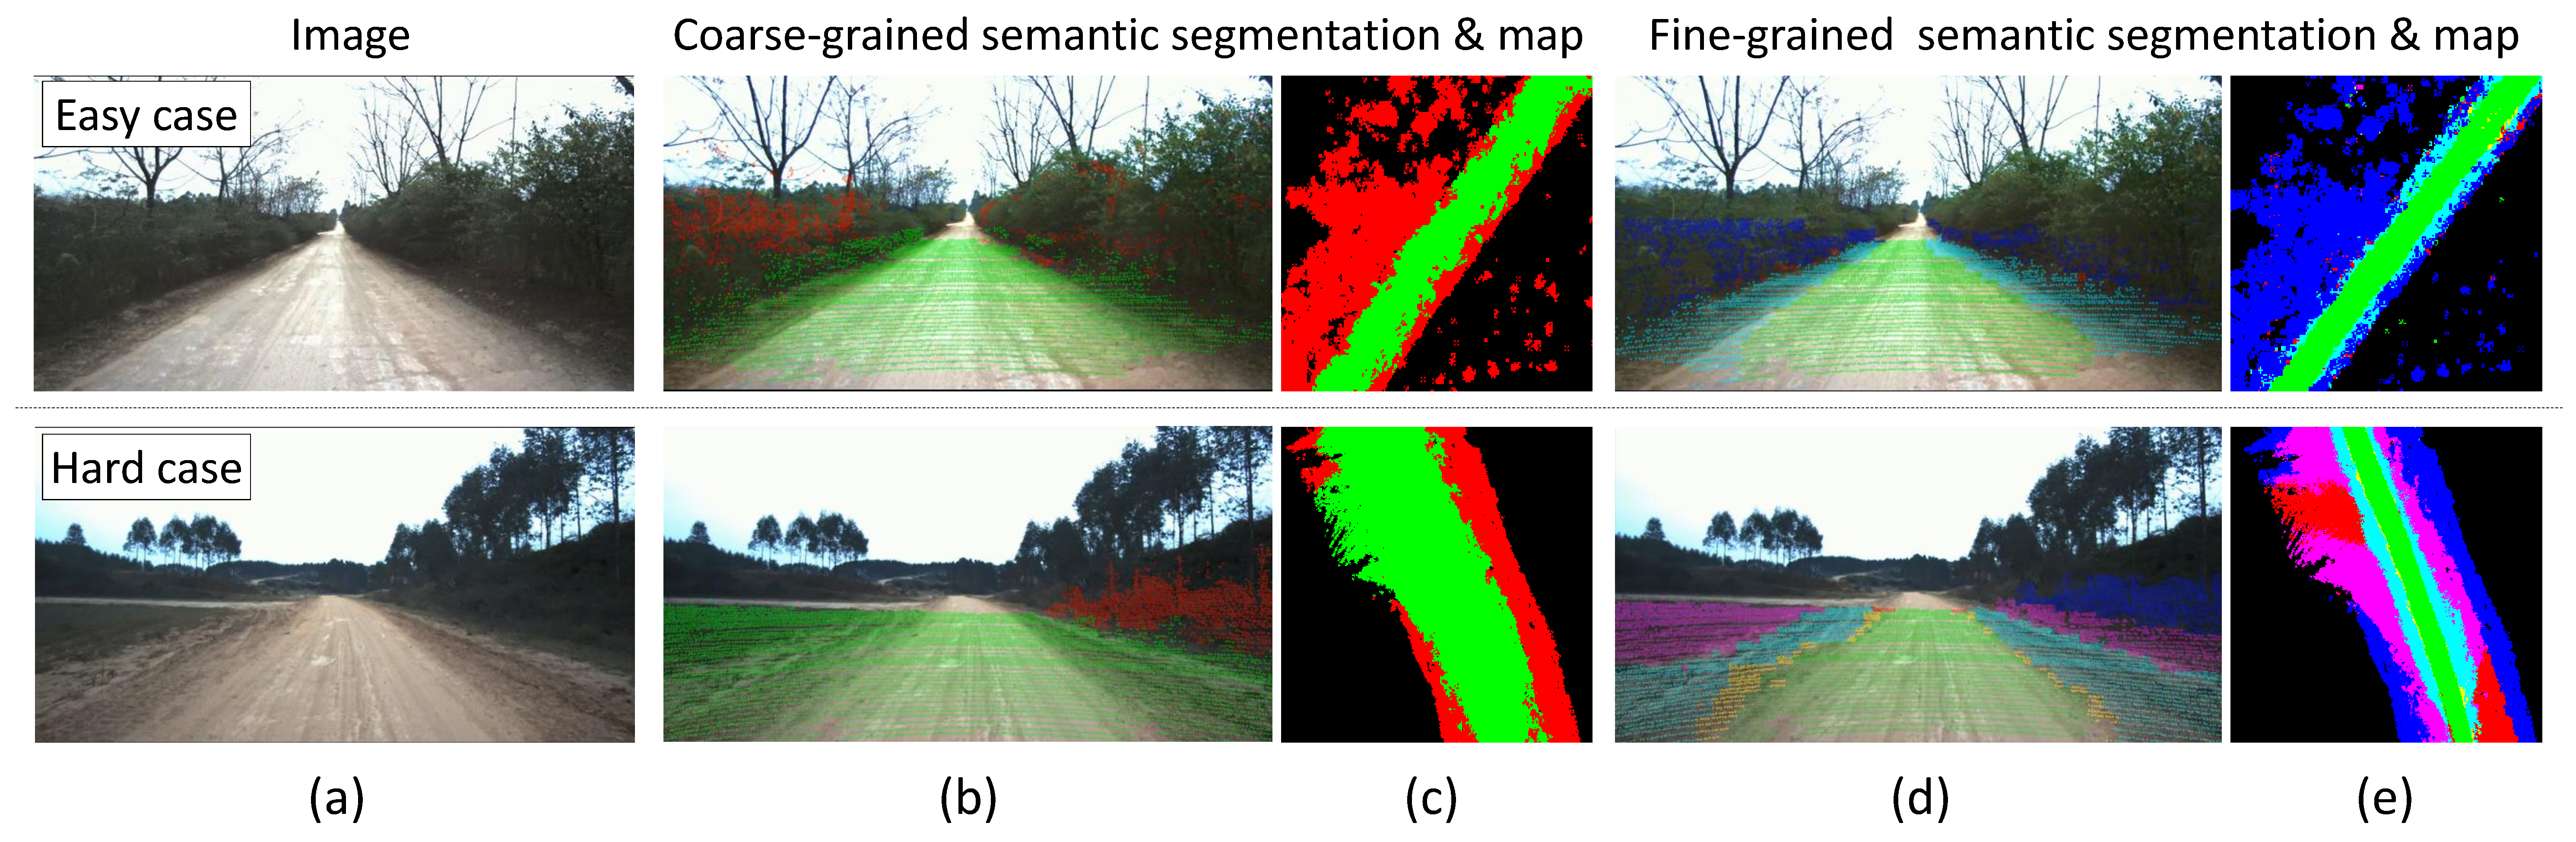
\includegraphics[width=\textwidth]{problem_def.pdf}
			\captionof{figure}{The significance of fine-grained semantic segmentation and mapping in off-road environment, where coarse-grained results can hardly adapt diverse scenes with unified threshold. (a) scene image. (b) coarse-grained semantic segmentation (binary classification). (c) coarse-grained bird's-eye-view semantic map. (d) fine-grained semantic segmentation. (e) fine-grained bird's-eye-view semantic map.}
			\label{fig:problem_def}
			%        \vspace{3mm}
		\end{center}
	}]
}

\maketitle
\thispagestyle{empty}
\pagestyle{empty}


%%%%%%%%%%%%%%%%%%%%%%%%%%%%%%%%%%%%%%%%%%%%%%%%%%%%%%%%%%%%%%%%%%%%%%%%%%%%%%%%

\begin{abstract}

empty.

\end{abstract}


%%%%%%%%%%%%%%%%%%%%%%%%%%%%%%%%%%%%%%%%%%%%%%%%%%%%%%%%%%%%%%%%%%%%%%%%%%%%%%%%
\section{Introduction}
%近年来,无人驾驶技术迅猛发展。驾驶场景的语义理解,是无人车进行有效决策规划和自主行驶的前提。目前,面向城市场景的语义理解研究非常丰富。然而,越野场景以自然物体为主、缺少结构化特征的属性,使得这一问题的定义不够明确。
Recent years, a considerable development has grown up around the theme of intelligent vehicles. Driving scene understanding plays a critical role in the preconditions of decision planning and self-driving. For the moment, a considerable amount of studies for urban scenes has been published. However, the off-road environment mainly consists of natural objects and lacks structured features, leading to ambiguous definition of this problem.
%不同类型的无人平台通行能力不同,细粒度的分类描述了不同的通行代价。比如图1所示的场景,如何提取无人平台可行驶的区域?如何评价不同区域的通行代价?回答这些问题,都需要对场景细粒度的语义理解。但是,越野场景的特殊性使这些问题至今仍缺乏明确的定义和公认的标准。
Different self-driving platforms have diverse trafficability, while the fine-grained semantic understanding could help to distinguish driving areas with diverse traversability cost. When facing off-road scenarios like Fig. \ref{fig:problem_def}(a), how to extract appropriate drivable area for self-driving platforms? How to evaluate traversability cost of different regions? To answer these questions, fine-grained semantic understanding is in great request. However, the particularity of off-road environment results in lack of clear definition and widely recognized standards.

%\textbf{已有相关的研究}可以分为传统方法和基于深度学习的方法
%\textbf{传统方法}:通常基于几何/视觉特征提取场景语义[ref],但是需要依赖人工定义的特征和经验参数,精度和性能有限;
%\textbf{深度学习方法}:借助深度网络提取更强的特征表达[ref],但是对监督样本的需求很大; 越野场景中,由于没有明确的问题定义,导致细粒度的人工标注非常困难。
%\textbf{对比学习}: 近年在视觉领域有很多研究,其算法优势是在无监督的情况下,可以学得高效的特征提取,并支撑ImageNet等语义类别粒度非常细致的图像分类任务。

Existing researches can be classified as traditional methods and deep learning methods.
Traditional methods mainly make use of geometrical and visual features to extract semantic meanings, but usually depend on manual defined features and empirical parameters, limiting its performance. As shown in Fig. \ref{fig:problem_def}(b-c), traditional methods may be in trouble when facing diverse scenarios. With uniform parameters, the drivable area may be too wide to provide human preferred area at flat scene, while cannot extract consecutive drivable area at rugged scene. Expected fine-grained semantic segmentation as shown in Fig. \ref{fig:problem_def}(d-e) could extract different semantic regions in different scenes, which improves the traversability analysis ability for off-road driving.
Deep learning methods depend on deep networks to obtain better feature representations, but rely heavily on massive annotated data. In off-road environments, the ambiguous problem definition leads to difficulty and scarcity of human annotations.
Several attempts about contrastive learning have been made in computer vision researches, which can learn effective feature representations through self-supervised pipeline. It has been proved to support fine-grained image classification tasks in large-scale datasets like ImageNet\cite{deng2009imagenet}.

%为了解决越野场景细粒度语义理解面临的困难(定义不明确、且缺少细粒度标注数据),本文提出了一个基于对比学习的面向越野环境细粒度语义聚类的方法。
%相比传统方法,我们利用对比学习自动地提取特征表达
%同时,仅需要少量简单的锚点标注,就可以得到细粒度的语义聚类结果。有效缓解了深度网络对细粒度人工标注的需求。
%我们通过......的实验证明了该方法的有效性.
To solve the challenges in fine-grained off-road semantic segmentation, i.e. ambiguous problem definition and the scarcity of elaborate annotated datasets, this work proposed a fine-grained off-road semantic segmentation method based on contrastive learning techniques. Compared with traditional methods, the proposed framework can automatically learn feature representations through contrastive learning. Meanwhile, only a small number of anchor annotations are required to get fine-grained semantic segmentation results, which significantly reduce the deep network's demand of laborious human annotations. The experimental results prove the validity of our proposed method, and show its potential in applications like semantic mapping.

%本文结构如下…
This paper is organized as follows. First, the related works
are introduced in Section \ref{related_works}. Section \ref{methodology} presents the proposed methodology in detail. Section \ref{exp} shows experimental results. Finally, we draw conclusions in Section \ref{conclusions}.

\section{Related Works} \label{related_works}
\subsection{Traditional Methods}
Rule-based: 消失点, 三角形/梯形;
Segmentation-based: AdaBoost, SVM, GMM

\subsection{Deep Learning Methods}
FCN, IV-19等

\subsection{Contrastive Learning}
CMC, MoCo, SimCLR

\section{Methodology} \label{methodology}
\begin{figure*}[]
%	\vspace{-2mm}
	\centering
	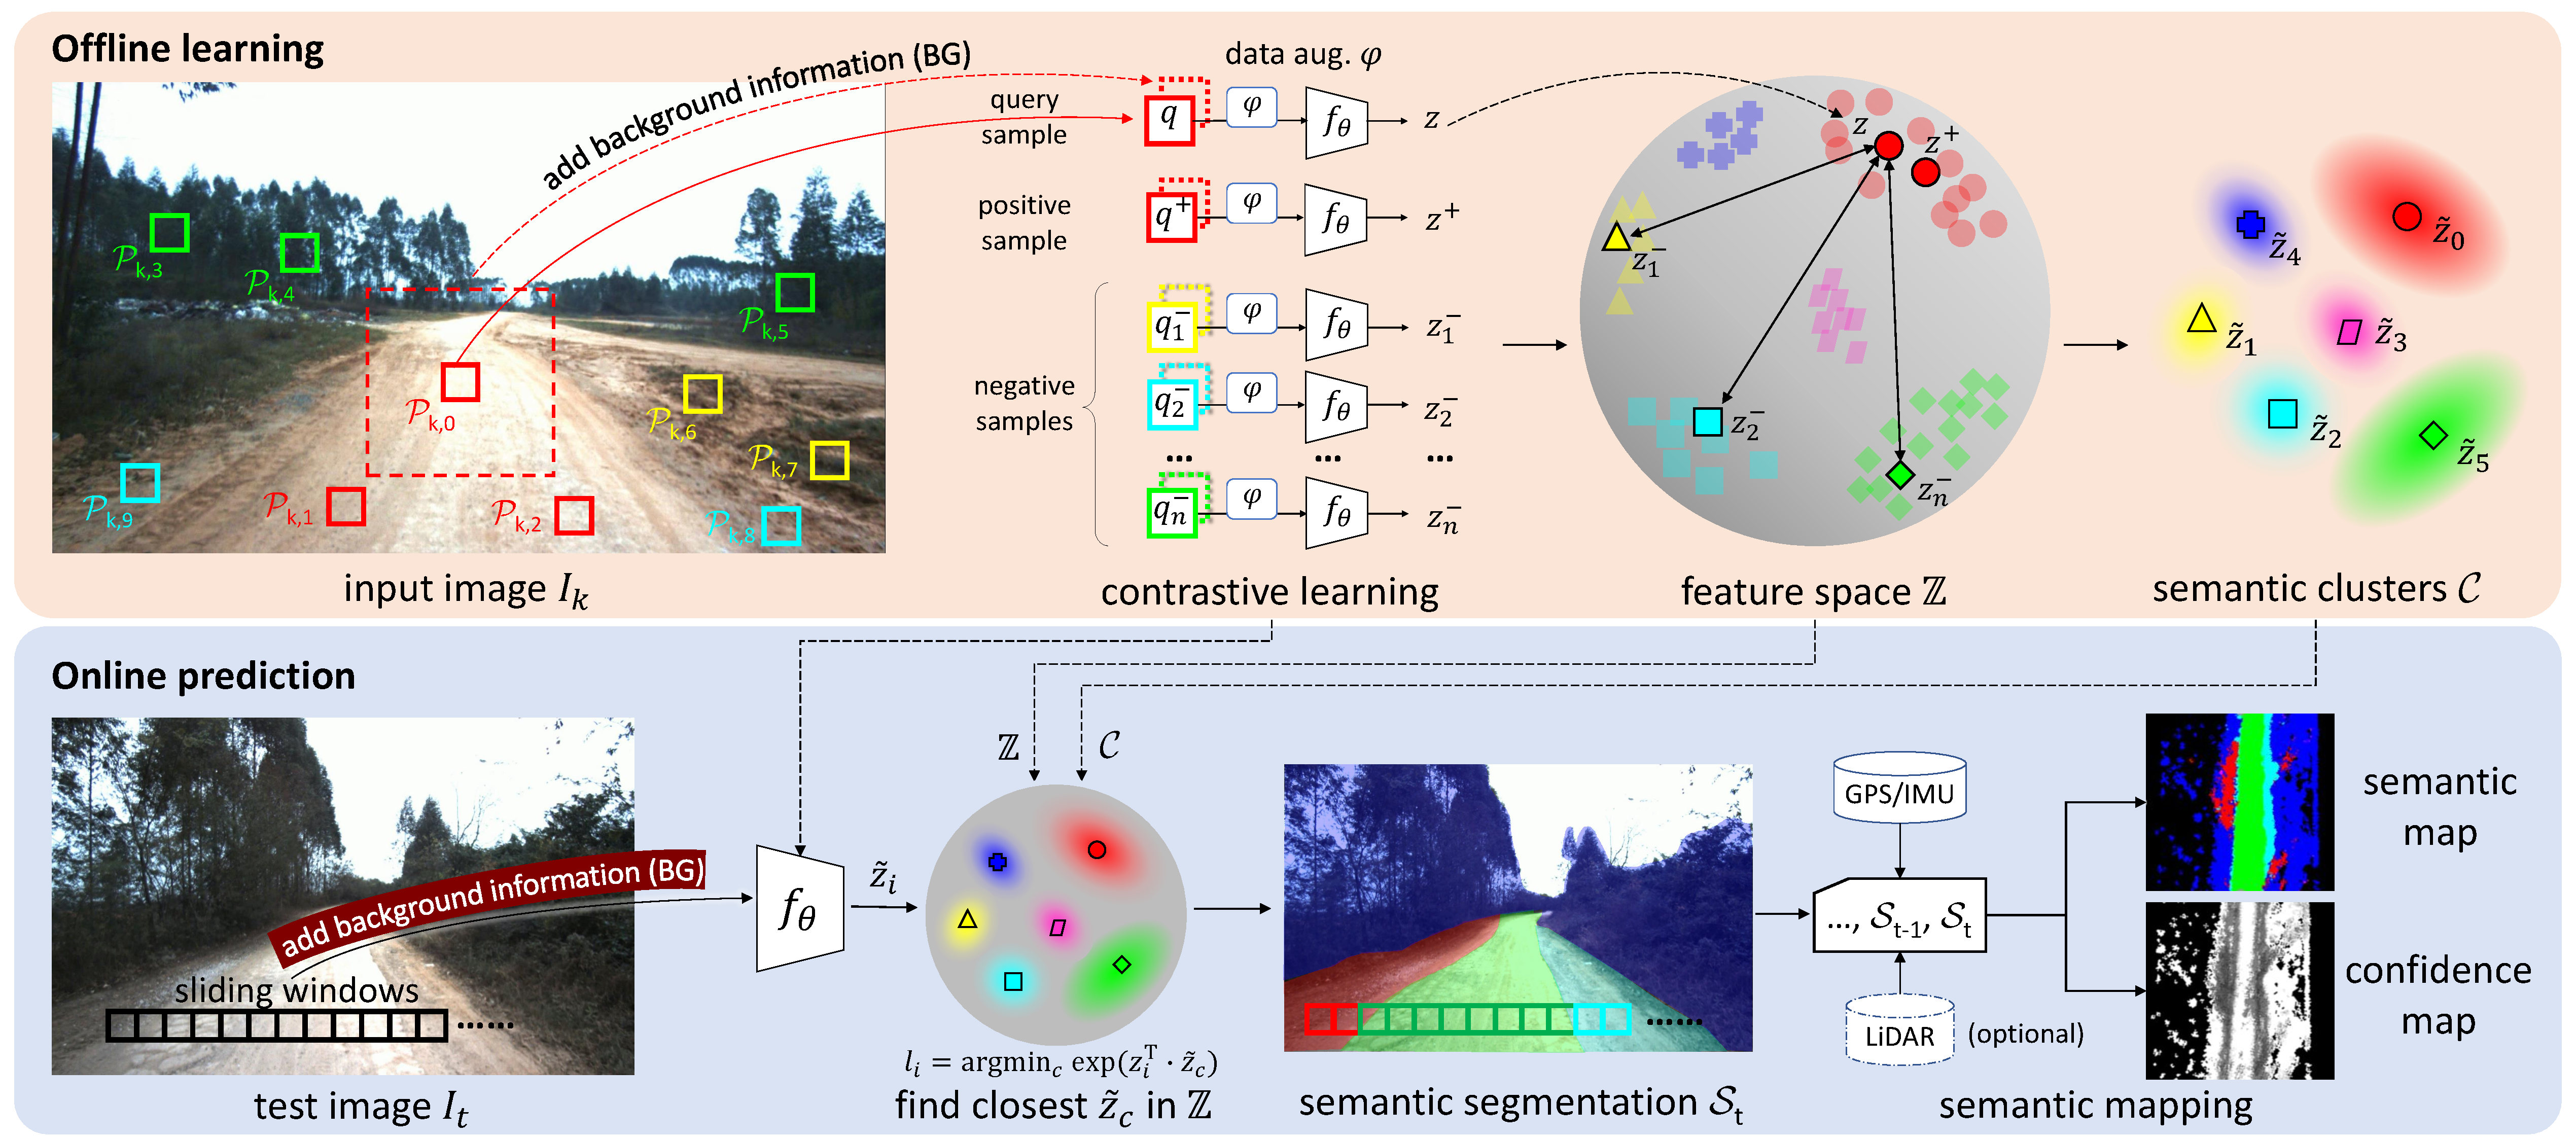
\includegraphics[scale=0.24]{pipeline.pdf}
	\caption{The proposed pipeline for fine-grained off-road semantic segmentation via contrastive learning.}
	\label{fig:pipeline}
\end{figure*}
\subsection{Problem Formulation}

A training image $I_k$ has a number of anchor patches $A_k=\{\mathcal{P}_{k,i}=<p_{k,i},a_{k,i}>\}$, where an anchor patch $\mathcal{P}_{k,i}$ is a pair of an image patch $p_{k,i}$ and a label $a_{k,i}$. Here, $a_{k,i}$ has no semantic meaning, but is an identifier of the image patches with similar or different semantic properties.
Let $z=f_{\theta}(p)$ be an encoder converting a high-dimensional image patch $p$ to a low-dimensional feature vector $z\in \mathbb{Z}^D$. 
We use exponential cosine distance $d(p_i,p_j)=exp(z_i^T \cdot z_j)$ to measure the similarity of two image patches via their low-dimensional feature vectors.
Therefore, given an image patch $\mathcal{P}_{k,i}$, its distance to another image patch $\mathcal{P}_{k,j}$, i.e. $d(p_{k,i},p_{k,j})$, should be smaller if they share the same label $a_{k,i}=a_{k,j}$, whereas larger if the labels are different $a_{k,i} \neq a_{k,j}$.
In order to make the annotation operational easy, in this research, the labels of the anchor patches are comparable only if they belong to the same image.

Given a set of training images $\mathcal{I}=\{I_k\}$ with anchor patches $\mathcal{A}=\{A_k\}$ on each of them, this research is to find a representation $f_{\theta}$ that encodes image patch $p$ to $z$, where at the low-dimensional feature space $\mathbb{Z}^D$, the $z$s of similar semantic meaning distribute closely. 
This research finds $f_{\theta}$ through contrastive learning, which is further used in an application of fine-grained semantic segmentation for off-road traversability analysis.
\subsection{Feature Representation through Contrastive Learning}

\subsubsection {Sampling strategy}
%In each training step, an anchor patches $\mathcal{P}_{k,i}$ is selected to compose a query sample $q$, and anchor patches with the same label as $\mathcal{P}_{k,i}$ are denoted as $\{\mathcal{P}_{k,i}^+\}$. Assuming that an image of the scene is spatially continuous, i.e. nearby regions could be semantically similar, an image patch is randomly sampled from $\mathcal{P}_{k,i}$'s and $\{\mathcal{P}_{k,i}^+\}$'s neighbors to compose a positive sample $q^+$. Meanwhile, $n$ negative samples $\{q^-\}$ are composed by randomly selecting the anchor patches of different label or sampling from their neighborhood. As shown in Fig. \ref{fig:dataaug}(a), sampled neighbors' centers are inside the origin anchor patch, to maintain spatial continuity.
In each training step, an anchor patch $\mathcal{P}_{k,i}$ is selected to compose a query sample $q$, and a positive sample $q^+$ and $n$ negative samples $\{q^-_i|i=1,..,n\}$ are subsequently composed on the anchor patches of the same image $I_k$.

Based on the label $a_{k,i}$ of $\mathcal{P}_{k,i}$, the anchor patches of the same image $I_k$ are divided into two sets, where $\{\mathcal{P}_{k,i}^+\}$ denotes those sharing the same label $a_{k,i}$, whereas $\{\mathcal{P}_{k,i}^-\}$ for the rest.
Assuming that an off-road scene is spatially continuous, i.e. nearby regions could be semantically similar.
An anchor patch is first selected randomly from $\{\mathcal{P}_{k,i}^+\}$, where an image patch is randomly clipped from its neighborhood to compose a positive sample $q^+$. As illustrated in Fig. \ref{fig:dataaug}(a), the neighborhood is defined to have the center point of the randomly clipped image patch within the original one. Similarly, $n$ negative samples $\{q^-_i\}$ are composed on $\{\mathcal{P}_{k,i}^-\}$.

\subsubsection{Composing sample data}

\begin{figure}[]
	%	\vspace{-2mm}
	\centering
	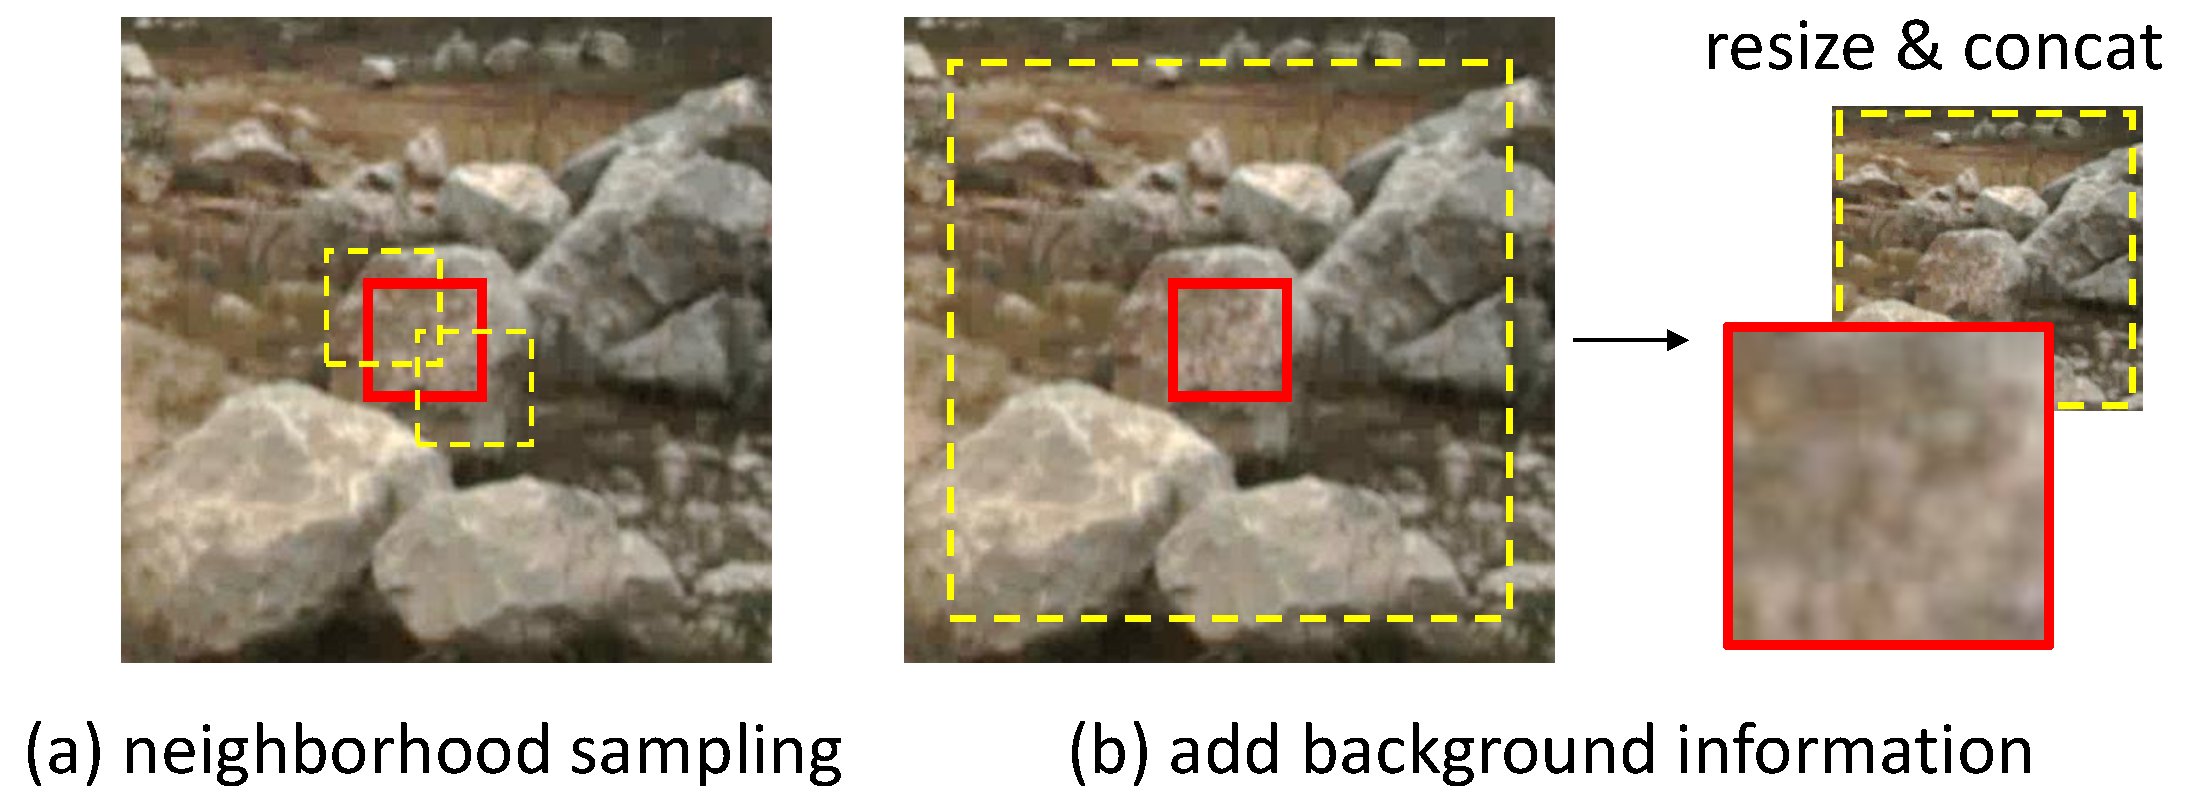
\includegraphics[scale=0.235]{dataaug.pdf}
	\caption{Illustration of (a) neighborhood sampling strategy, and (b) how to add background information with the origin image patch.}
	\label{fig:dataaug}
\end{figure}
%In order to enrich the diversity of input samples and train a robust feature encoder, data augmentation $\phi$ will be implemented to the query sample $q$, its positive sample $q^+$ and negative samples $\{q^-\}$, before fed to the encoder network.
%The basic data augmentation includes commonly used random flip, grey scale and color jitter, which randomly change the brightness, contrast and saturation of an image.
%In addition, we propose to add background information as an advanced data augmentation, shown in Fig. \ref{fig:dataaug}(b). One anchor patch and its concentric larger-size background patch will be resized to the same scale and concatenated along the channel dimension to get a 6-channel tensor. Depending on different augmentation settings, the image patch of query sample $q$ could be a common 3-channel image or a 6-channel tensor including both foreground and background image patches.
With an image patch $p$, a sample data is composed in the same way for query, positive or negative samples.
As shown in Fig. \ref{fig:dataaug}(b), a sample data contains foreground and background image patches to describe both local and global features. Foreground is image patch $p$, while background is centered at $p$ but with a larger region to provide global scene context. The foreground and background patches are firstly resized to the same scale, then the two patches are concatenated along the channel dimension to compose a 6-channel tensor.

In order to improve robustness in diverse scenes, data augmentation (denoted by $\phi$ in Fig. \ref{fig:pipeline}) is conducted on the 6-channel tensor of each sample data before forwarding it to the network of $f_{\theta}$. In this research, data augmentation includes random flip, random grey scale and color jitter, which randomly changes the brightness, contrast and saturation of an image.

\subsubsection{Network Design and Loss Function}
%After data augmentation, the sample $q$ will be taken as input of the feature encoder $f_{\theta}$, which is a CNN backbone network in practical terms, e.g., AlexNet\cite{krizhevsky2012imagenet}. The backbone network's output is a latent feature vector $z\in \mathbb{Z}^D$. By the way, unlike some typical contrastive learning studies\cite{Wu_2018_CVPR} using memory bank to store latent features for each training sample, we randomly select positive/negative samples and calculate their features at each training step. Because in this work, the positive and negative samples are comparable only in the same image, the limited quantity makes it possible to get the latest feature representations with reasonable memory consumption.

A CNN backbone network in practical terms, e.g. AlexNet[2] is used to model $f_{\theta}$, which converts the 6-channel tensor of a query, positive or negative sample to a low-dimensional feature vector $z\in \mathbb{Z}^D$.
Contrastive learning is used to find a $\theta$ of $f_{\theta}$, with which the exponential cosine distance of the $z$s are close if they share the same labels, whereas far for those different.
Following the principle of previous contrastive learning studies, a contrastive loss function InfoNCE\cite{oord2018representation} is implemented:

\begin{equation}\label{loss}
L=-\log {\dfrac{\exp (z^T \cdot z^+/\tau)}{\exp (z^T \cdot z^+/\tau)+\sum_{i=0}^{n}{\exp (z^T \cdot z_i^-/\tau)}}}
\end{equation}
where $\tau$ denotes a temperature hyper-parameter.

\subsection{Fine-grained Off-road Semantic Segmentation}
\subsubsection{Pipeline}
The pipeline is shown in Fig. \ref{fig:pipeline}. In training stage, the feature encoder $f_\theta$ is trained through contrastive learning. Then, all training image patches' will be clustered in the latent feature space $\mathbb{Z}$ and get some category clusters $\mathcal{C}=\{c_i\}$.
When predicting, given an image $\mathcal{I}$, we use sliding windows to get query patches, then project them into feature space $\mathbb{Z}$ and classify into existing category clusters $\mathcal{C}$. Therefore, each patch will get a category label and constitute semantic segmentation results.

\subsubsection{Clustering and Semantic Segmentation} \label{3_CSS}

We use K-means algorithm for category clustering of all anchor patches in training set. Exponential cosine distance $d(p_i,p_j)=exp(z_i^T \cdot z_j)$ is used to evaluate distances between image patches. By the way, the clustering number $\mathcal{K}$ is assigned by human, which decides category granularity.

When predicting dense semantic segmentation, patches' corresponding latent features are projected to feature space $\mathcal{Z}$ through $f_\theta$. The semantic label will be assigned by the closest cluster center. To make up denser semantic segmentation, we could adjust step size of sliding windows. For example, we can assign the semantic label to $3*3$ pixels centered at each image patch, while setting sliding windows' horizontal/vertical step size to 3 pixels, then get denser semantic segmentation results.

To evaluate the overall performance and consistence of the fine-grained prediction on continuous video frames, we project the semantic segmentation of images to corresponding LiDAR point clouds, and utilize GPS/IMU information to make semantic maps. Testing of continuous video frames will lead to multiple predictions of the same pixel on the semantic map. Let $\sigma_c$ denote the counts of prediction with label $c$, then the pixel label in semantic maps will be $l=\mathop{\text{argmax}_{c} (\sigma_c)}$. Confidence map indicates the predictions' consistency, where each pixel's value is $\max(\sigma_c)/\sum{\sigma_c}$.

\section{Experimental Results}	\label{exp}
\subsection{Dataset}
The performance of our proposed method is evaluated on the off-road dataset, called \textit{GL-Offroad}. The dataset is collected by an instrumented vehicle with a front-view monocular camera, a GPS/IMU suite and a 3D LiDAR. In this work, we mainly use camera images as input data, while the GPS/IMU and LiDAR data are supplementary for semantic mapping.
As shown in Table \ref{tab:dataset}, the \textit{GL-Offroad} dataset includes 3 subsets. Take subset A as an example, we randomly selected 50 frames for 973 anchors annotation and training, which only account for about $10\%$ of total 5064 frames. While all frames are evaluated when testing, and frames with human annotations are taken into account in quantitative evaluation.

In addition, as shown in Fig. \ref{fig:dataset}, the 3 subsets represent different typical off-road environments. The scenarios in subset A are mostly narrow roads with bushes aside. Subset B are relatively wide scenes, and subset C includes diverse scenarios like slimy path in woodland and flatland without road structure. In following experiments, we train and test the proposed method on different subsets to evaluate its cross-scene generalization performance.

\begin{table}[h]
	\centering
	\caption{Statistics of \textit{GL-Offroad} dataset}
	\label{tab:dataset}
	\begin{tabular}{cccc} 
		\hline
		& subset A & subset B & subset C  \\ 
		\hline
		total frames        & 5064     & 3239     & 4098      \\
		frames for training & 50       & 100      & 80        \\
		anchors       & 973      & 1606     & 1437      \\
		\hline
	\end{tabular}
\end{table}

\begin{figure}[h]
	%	\vspace{-2mm}
	\centering
	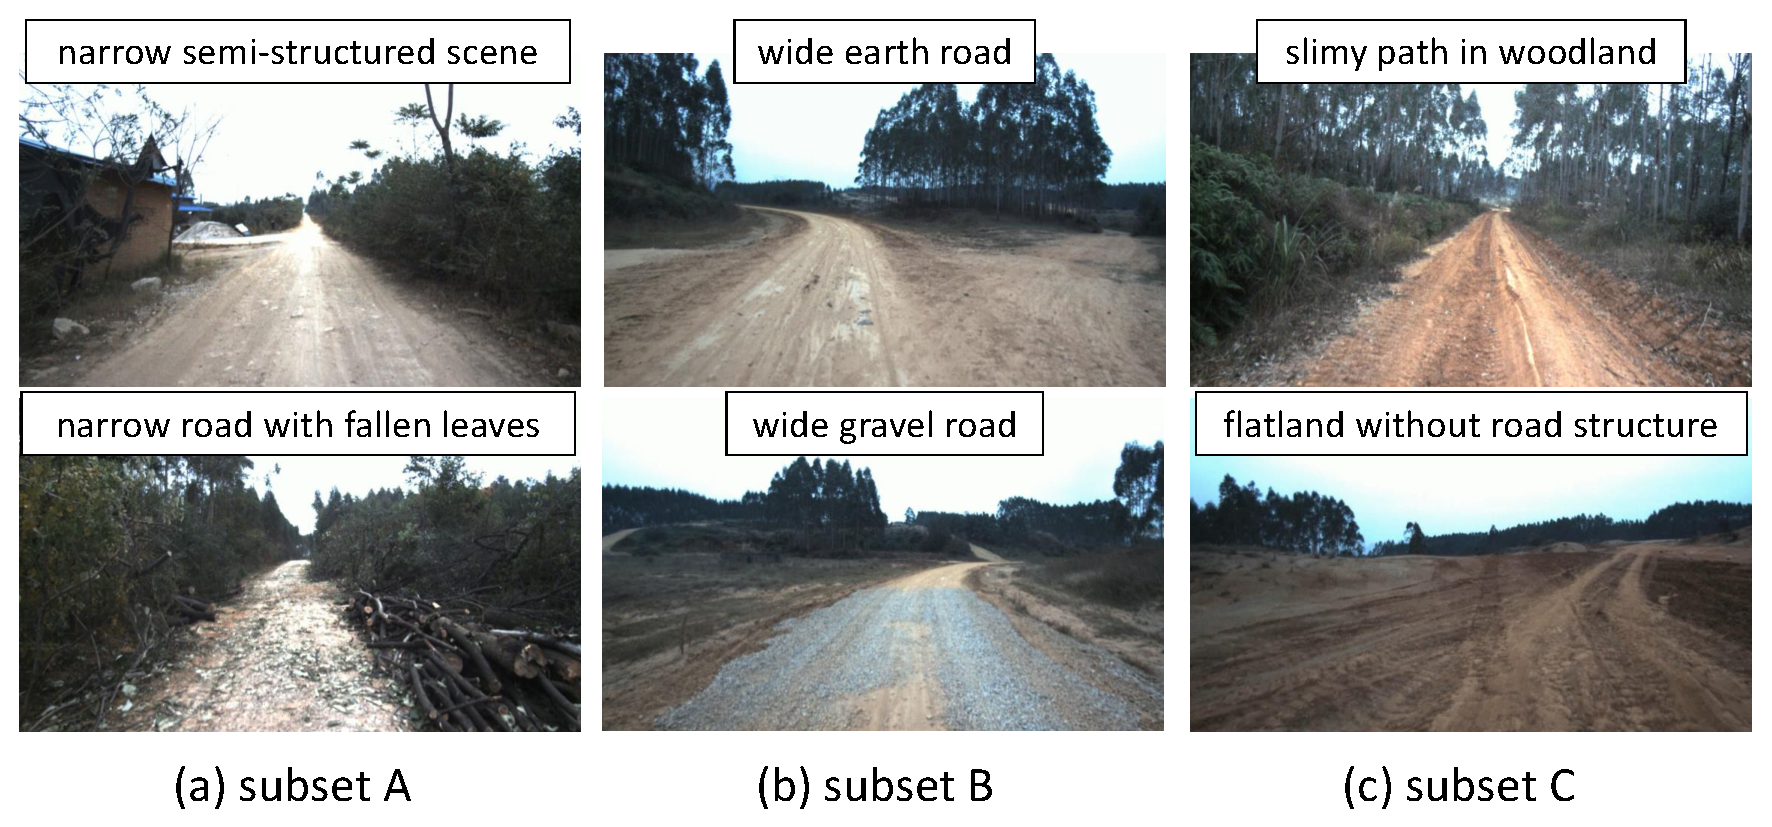
\includegraphics[scale=0.28]{dataset.pdf}
	\caption{Typical scenes in three datasets, which represent different off-road environments.}
	\label{fig:dataset}
\end{figure}

\subsection{Evaluation Metrics}
Suppose that there are $N$ anchors in one frame, then any two anchors must be either positive or negative samples of each other. Hence, there exists $N \cdot(N-1)$ pairs anchor constraints.
%假设一帧图像中有$N$个锚点,两两互为正/负样本,则存在$N\cdot(N-1)$对正负样本约束
We denote positive samples' constraints as $Pos(i,j)$: if anchor $a_i$ and $a_j$ are positive samples of each other and classified into the same cluster, $Pos(i,j)=1$. Otherwise, if they are not classified to the same cluster, $Pos(i,j)=0$.
Negative samples' constraints are defined in a similar way, and denoted as $Neg(i,j)$.
%正样本约束:若锚点$a_i$和$a_j$互为正样本,且聚类标签$Lab_i=Lab_j$,则满足正样本约束,并记$Pos(i,j)=1$,否则$Pos(i,j)=0$. 负样本约束$Neg(i,j)$定义同理;

\begin{figure*}[b]
	%	\vspace{-2mm}
	\centering
	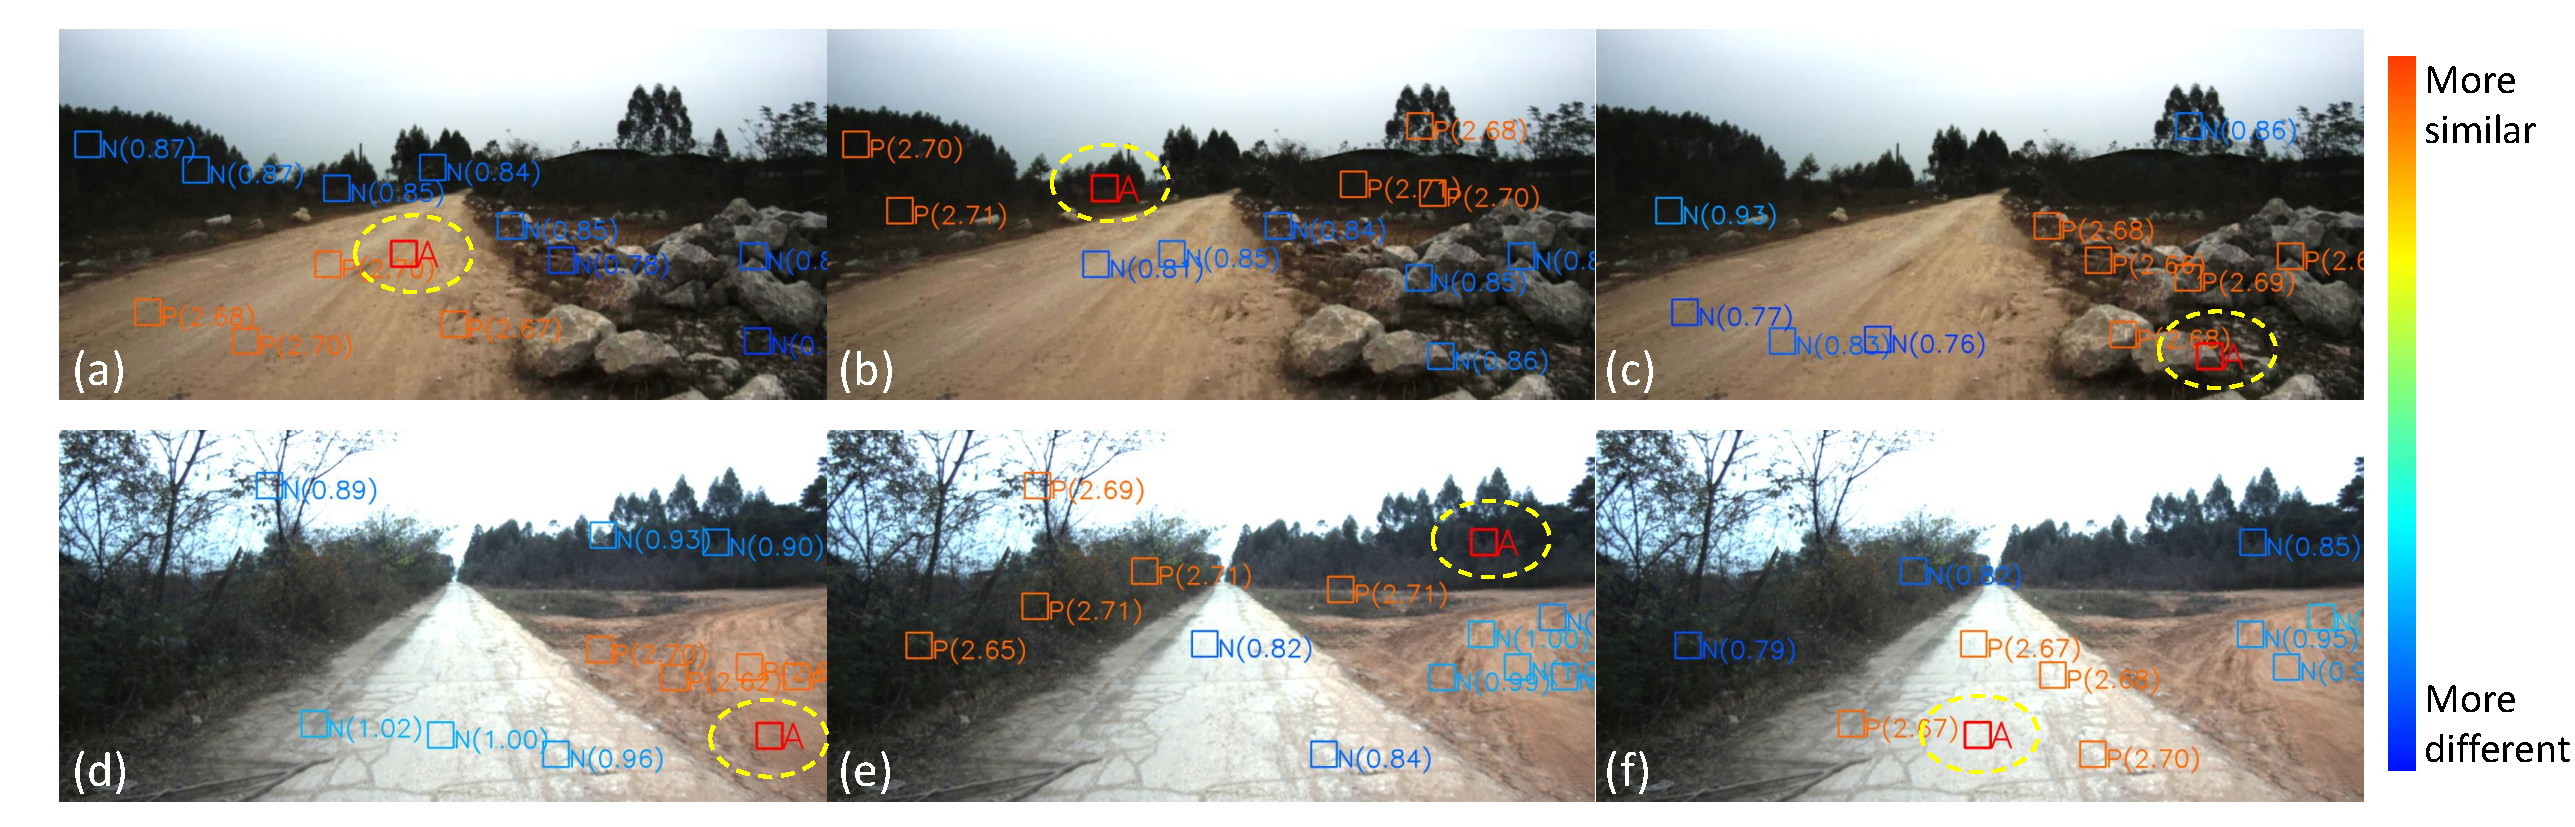
\includegraphics[scale=0.4]{anchor_dis.pdf}
	\caption{Visualization of feature distances of query anchor (A) to its positive (P) and negative (N) samples. Query anchors are circled by yellow rings. P/N is according to human annotated anchor labels, and numbers in parentheses measure samples' similarity to the query anchor.}
	\label{fig:anchor_dis}
\end{figure*}

We use the following metrics to evaluate how well the clustering results fit human annotated anchors:

\begin{equation}
\mathcal{R}=\dfrac{\sum_{i,j}{Pos(i,j)}+\sum_{i,j}{Neg(i,j)}}{N\cdot (N-1)}, i \neq j
\end{equation}
Essentially, it can be seen as Rand Index \cite{rand1971objective}, which is a common used measurement for clustering.

\begin{table*}
	\centering
	\caption{Cross Validation Results ($\mathcal{R}$) on Different Datasets}
	\label{tab:cross_eval}
	\renewcommand{\arraystretch}{1.2}
	\begin{threeparttable}
		\begin{tabular}{ccc|ccc|ccc|ccc!{\color{black}\vrule}c} 
			\hline
			\multirow{3}{*}{model} & \multirow{3}{*}{\makecell[c]{data\\ aug.}} & \multirow{3}{*}{\makecell[c]{BG\\ size}} & \multicolumn{3}{c|}{train on subset A}                                                                             & \multicolumn{3}{c|}{train on subset B}                                                                             & \multicolumn{3}{c|}{train on subset C}                                                                             & \multirow{3}{*}{\makecell[c]{$\bar{\mathcal{R}}$ on \\ test sets}}                      \\ 
			\cline{4-12}
			&                            &                             & \multicolumn{3}{c|}{test on}                                                                                       & \multicolumn{3}{c|}{test on}                                                                                       & \multicolumn{3}{c|}{test on}                                                                                       &                                                      \\
			&                            &                             & A      & B                                                   & C                                                   & B      & A                                                   & C                                                   & C      & A                                                   & \multicolumn{1}{c|}{B}                              &                                                      \\ 
			\hline
			base                   & $\times$                          & $\times$                           & 0.9854 & {\cellcolor[rgb]{1,0.906,0.906}}0.8548              & {\cellcolor[rgb]{0.992,0.722,0.722}}0.8509          & 0.9997 & {\cellcolor[rgb]{1,0.906,0.906}}0.7957              & {\cellcolor[rgb]{1,0.906,0.906}}0.8492              & 0.9966 & {\cellcolor[rgb]{1,0.906,0.906}}0.8288              & {\cellcolor[rgb]{0.992,0.745,0.749}}0.9258          & {\cellcolor[rgb]{1,0.906,0.906}}0.8509               \\
			base\_DA               & \checkmark                          & $\times$                          & 0.9693 & {\cellcolor[rgb]{0.996,0.773,0.773}}0.8792          & {\cellcolor[rgb]{1,0.906,0.906}}0.8422              & 0.9959 & {\cellcolor[rgb]{0.992,0.733,0.733}}0.8210          & {\cellcolor[rgb]{0.992,0.745,0.749}}0.8625          & 0.9913 & {\cellcolor[rgb]{1,0.898,0.898}}0.8296              & {\cellcolor[rgb]{1,0.906,0.906}}0.9119              & {\cellcolor[rgb]{0.996,0.835,0.835}}0.8578           \\
			BG192                  & \checkmark                          & 192                         & 0.9939 & {\cellcolor[rgb]{0.976,0.471,0.478}}0.9330          & {\cellcolor[rgb]{0.973,0.412,0.42}}\textbf{0.8650}  & 0.9994 & {\cellcolor[rgb]{0.98,0.514,0.518}}0.8524           & {\cellcolor[rgb]{0.973,0.412,0.42}}\textbf{0.8899}  & 0.9944 & {\cellcolor[rgb]{0.98,0.537,0.545}}0.8653           & {\cellcolor[rgb]{0.98,0.502,0.51}}0.9468            & {\cellcolor[rgb]{0.976,0.475,0.482}}0.8920           \\
			BG256                  & \checkmark                          & 256                         & 0.9987 & {\cellcolor[rgb]{0.976,0.455,0.463}}0.9360          & {\cellcolor[rgb]{0.976,0.463,0.471}}0.8627          & 0.9991 & {\cellcolor[rgb]{0.976,0.475,0.482}}0.8577          & {\cellcolor[rgb]{0.98,0.486,0.494}}0.8839           & 0.9934 & {\cellcolor[rgb]{0.98,0.525,0.533}}0.8665           & {\cellcolor[rgb]{0.976,0.451,0.459}}0.9512          & {\cellcolor[rgb]{0.976,0.467,0.471}}0.8930           \\
			BG320                  & \checkmark                          & 320                         & 0.9986 & {\cellcolor[rgb]{0.973,0.412,0.42}}\textbf{0.9433}  & {\cellcolor[rgb]{0.984,0.612,0.616}}0.8559          & 0.9980 & {\cellcolor[rgb]{0.973,0.412,0.42}}\textbf{0.8667}  & {\cellcolor[rgb]{0.976,0.42,0.427}}0.8895           & 0.9958 & {\cellcolor[rgb]{0.973,0.412,0.42}}\textbf{0.8776}  & {\cellcolor[rgb]{0.973,0.412,0.42}}\textbf{0.9544}  & {\cellcolor[rgb]{0.973,0.412,0.42}}\textbf{0.8979}   \\
			\hline
		\end{tabular}
		\begin{tablenotes}
			\footnotesize
			\item[*] \textbf{BG}: background; \textbf{base}: basic pipeline without data augmentation or background information; \textbf{base\_DA}: with basic data augmentation, without background information; \textbf{BG192/256/320}: complete pipeline with different background size.
		\end{tablenotes}
	\end{threeparttable}
\end{table*}
\subsection{Results on Proposed Method}
%说明一下三个实验设计的目的:1.探究对比学习学到的特征表达、距离度量是否有效;2.通过交叉验证说明我们设计的模型具有较优的性能和不同场景下的泛化能力;3.通过构建细粒度语义地图/置信度地图,结合case study和激光平整度统计分析,说明细粒度分类结果的有效性。
To evaluate the proposed method, we design the following experiments: (1) feature distance measurement, explore the validity of feature encoder and distance measurement learned by contrastive learning. (2) cross validation and ablation study, verify the performance and robustness of our proposed method in diverse test scenes, while explore the effects of different modules or parameters. (3) fine-grained semantic segmentation and mapping, analyze the fine-grained semantic predictions through case study and semantic mapping, to show the method's validity for fine-grained off-road traversability analysis.


\subsubsection{Feature Distance Measurement}
%\textbf{回答问题}:对比学习模块学到的特征距离度量是否有效?\textbf{结论}:对比学习学到的特征距离度量,可以满足“语义相似的patch特征距离更近,语义不同的patch特征距离更远”的特性。
The core module in our proposed pipeline is the feature encoder $f_\theta$, which projects high-dimensional image patch to low-dimensional feature vector in space $\mathbb{Z}$. Its purpose is making feature distance closer between similar image patches, while farther between different image patches. In Fig. \ref{fig:anchor_dis}, we visualize some case studies. In all images, the query anchors are circled by yellow rings, while the other anchor patches are randomly sampled and colorized by its feature distance to the query anchor. For example, in Fig. \ref{fig:dataaug}(a), the query anchor is located on earth road. We can find that patches on earth road are closer to red, and other patches located on different semantic area are generally blue, which indicate farther distance to the query anchor. The feature distance distribution is accord with human annotated anchor labels. Similar situations are general on images (a)-(f). As a result, the learned feature encoder and distance measurement are able to distinguish similar or different image patches.

\begin{figure}[]
	%	\vspace{-2mm}
	\centering
	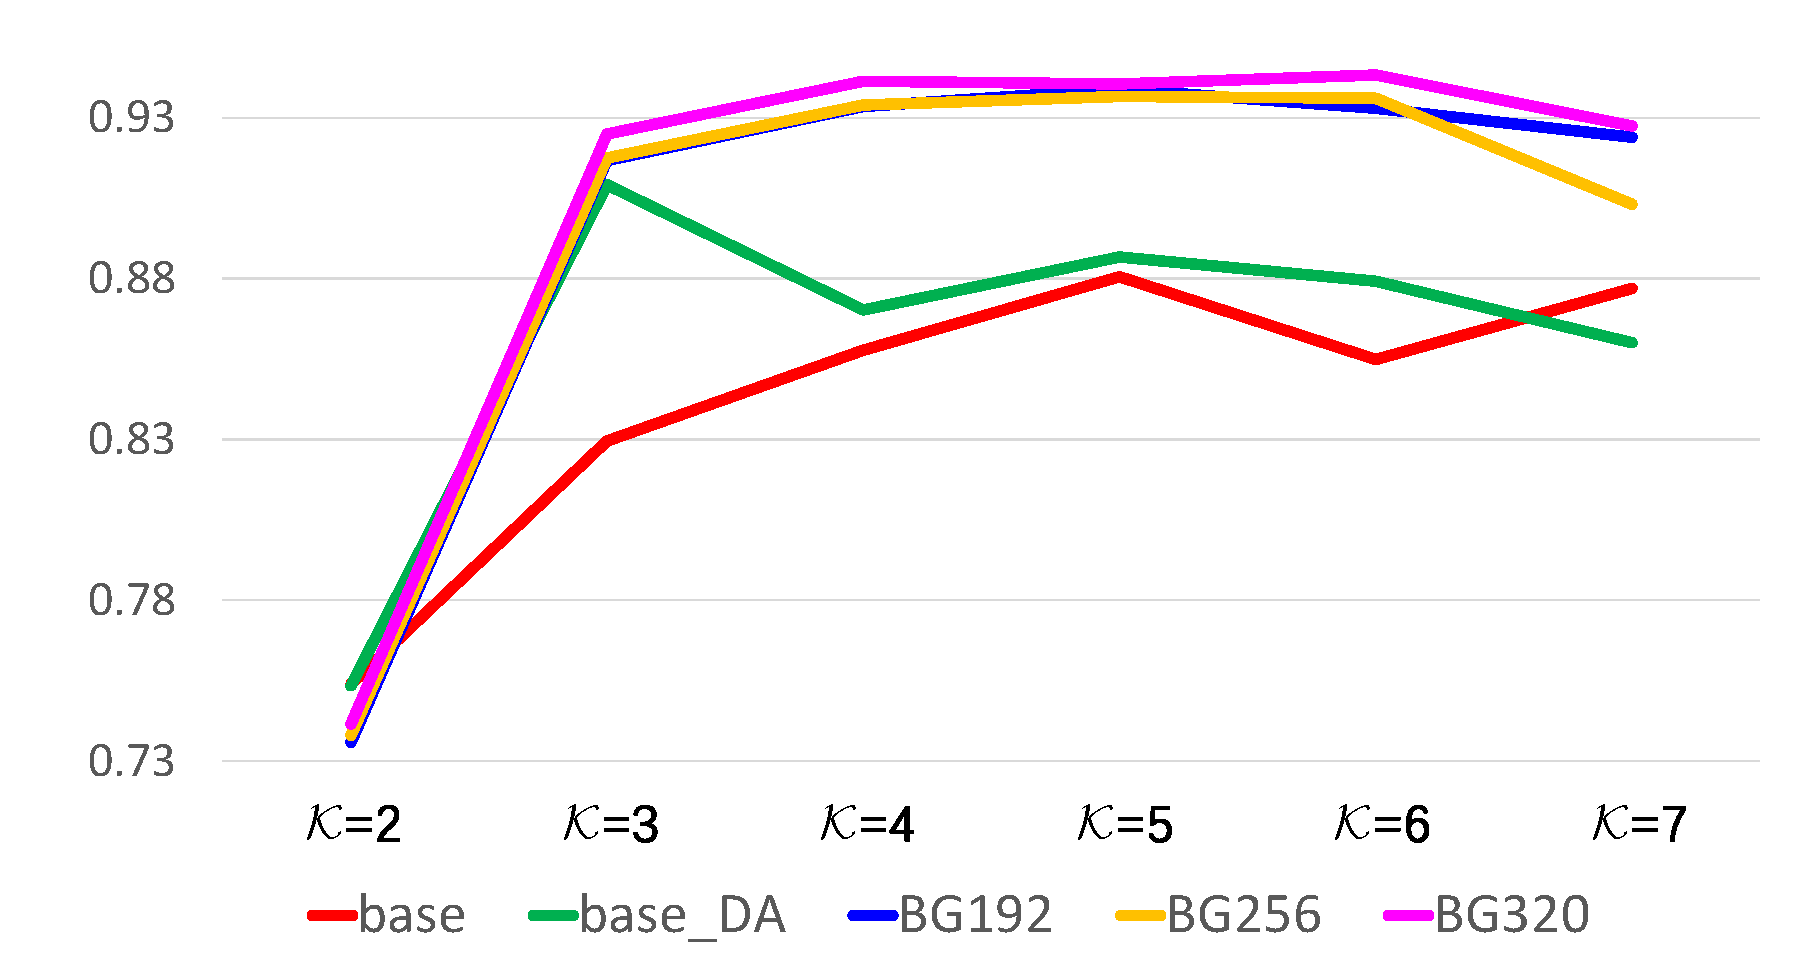
\includegraphics[scale=0.28]{kmeans_exp.pdf}
	\caption{Average $\mathcal{R}$ of models under different clustering number $\mathcal{K}$.}
	\label{fig:kmeans_exp}
\end{figure}

\subsubsection{Cross Validation and Ablation Study}

%\textbf{问题1}:我们的模型设计(数据增强+背景信息)是否性能较优,且在不同条件下有泛化能力?
%\textbf{结论1}:从表\ref{tab:cross_eval}中最后一列看出,BG320模型在测试集上具有最好的准确率;且加入了背景信息的3个模型在训练/测试集不同的情况下都可以达到0.85以上的准确率(泛化能力)。 说明我们的模型设计性能较优且有一定泛化能力。
%
%\textbf{问题2}:[Ablation Study 1]数据增强、背景信息分别起到了多少作用?
%\textbf{结论2}:从表\ref{tab:cross_eval}可以看出数据增强和背景信息都有作用,添加背景带来的性能提升更大;背景尺寸的增加带来略微提升,不显著;
%
%\textbf{问题3}:[Ablation Study 2]聚类数量K对结果的影响如何?
%\textbf{结论3}:从图\ref{fig:kmeans_exp}看出,聚类数量的变化会略微影响锚点吻合度, 但不是决定因素。整体来看,不同模型的性能排序与结论1一致。
For comprehensive evaluation of the proposed method, we make cross validation on models with different settings, and the statistics of $\mathcal{R}$ are shown in Table \ref{tab:cross_eval}. The table cells are colorized by column data, when training and testing on different subsets. The last column lists the average performance $\bar{\mathcal{R}}$ of models on test sets (different subsets with the training one). It is obviously that \textit{BG320} has the best performance on test sets, and all three models with background information have $\mathcal{R}$ over 0.85 among all training/testing combinations, which demonstrates the robustness of our proposed method.

Comparing the basic data augmentation with background information, they can both increase models' performance, while the latter makes more contribution. Besides, increasing background size could sightly improve the overall performance, but not obvious at all situations.

By the way, above experiments uniformly used clustering number $\mathcal{K}=6$. How does clustering number affects models' performance? An ablation study of $\mathcal{K}$ is made, and the results are shown in Fig. \ref{fig:kmeans_exp}. We can find that the models' performance with regard to $\mathcal{K}$ are basically stable when $\mathcal{K} \geq 4$, and slightly decrease when $\mathcal{K}>6$. In general, models' performance with different $\mathcal{K}$s approximately order the same as Table \ref{tab:cross_eval}. Therefore, we choose $\mathcal{K}=6$ as other experiments' setting, which balances the fine-grained demand and model performance.

\begin{figure*}[]
	%	\vspace{-2mm}
	\centering
	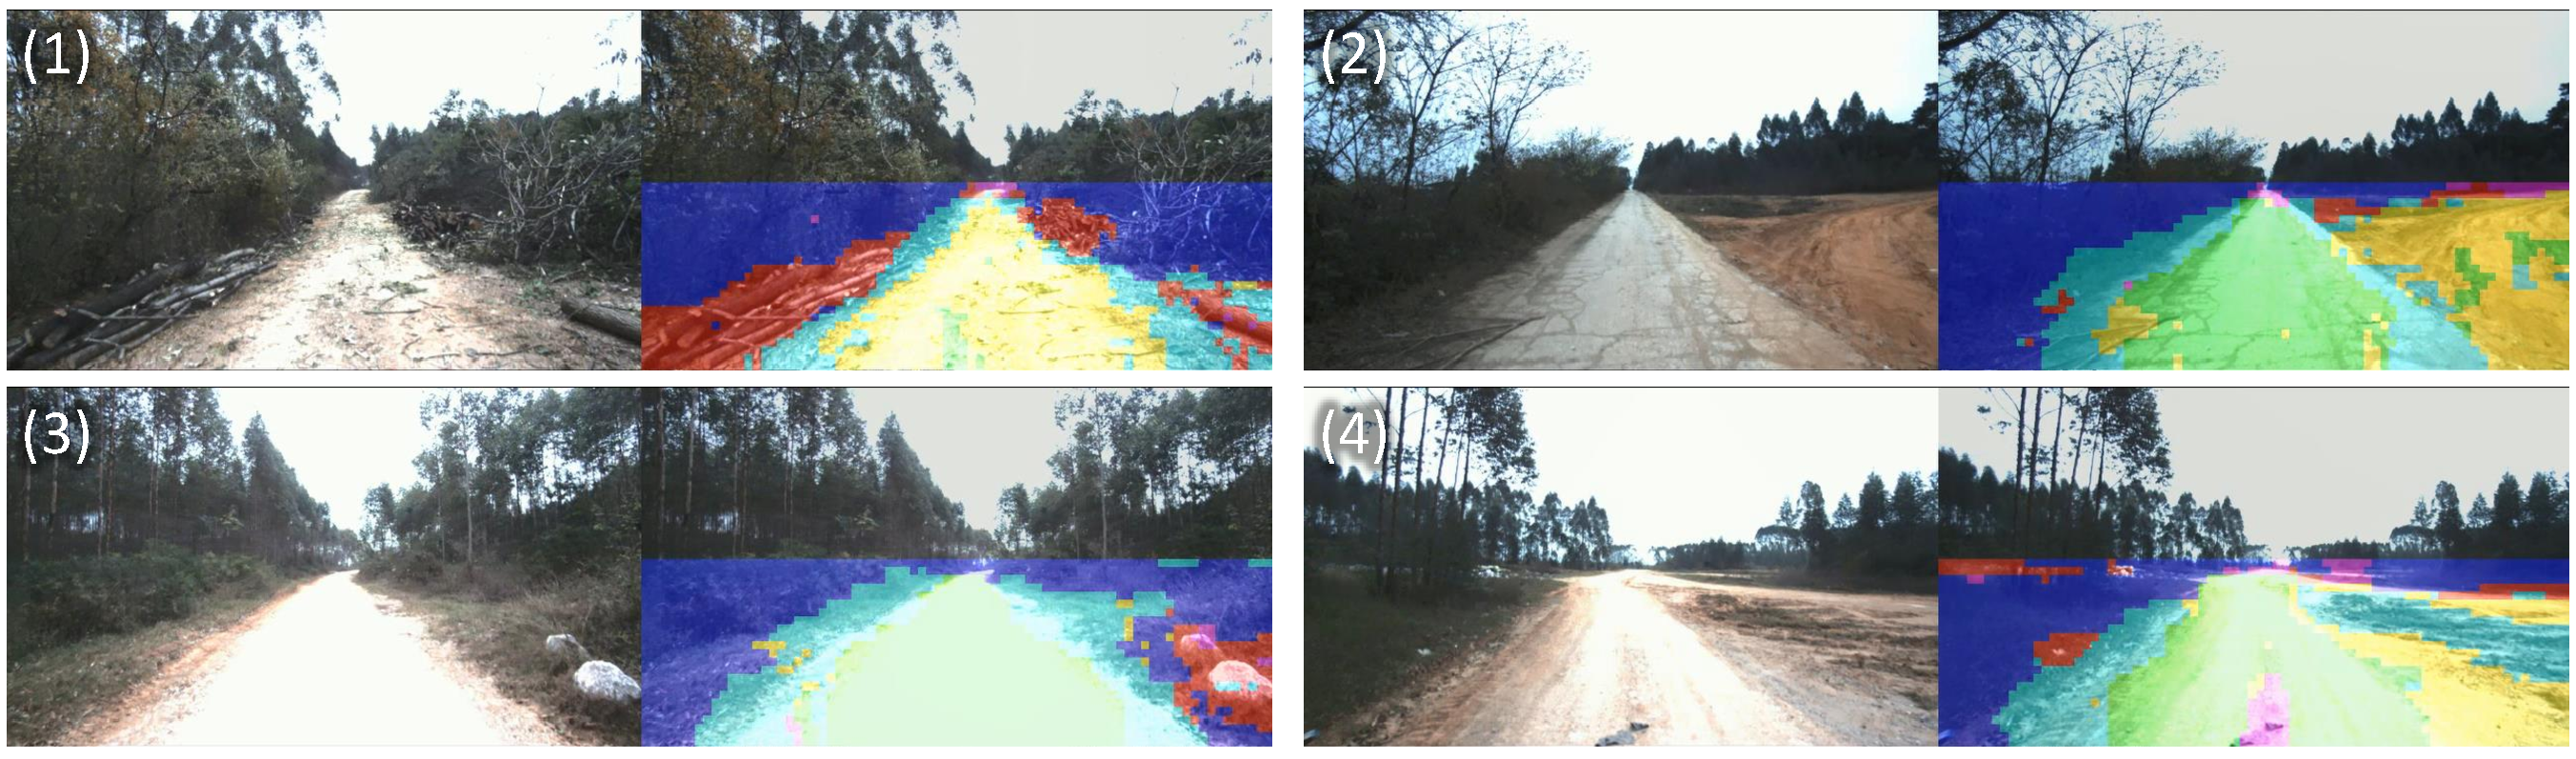
\includegraphics[width=0.95\textwidth]{semantic_segmentation.pdf}
	\caption{Some cases of fine-grained semantic segmentation.}
	\label{fig:semantic_segmentation}
\end{figure*}

\begin{figure*}[]
	%	\vspace{-2mm}
	\centering
	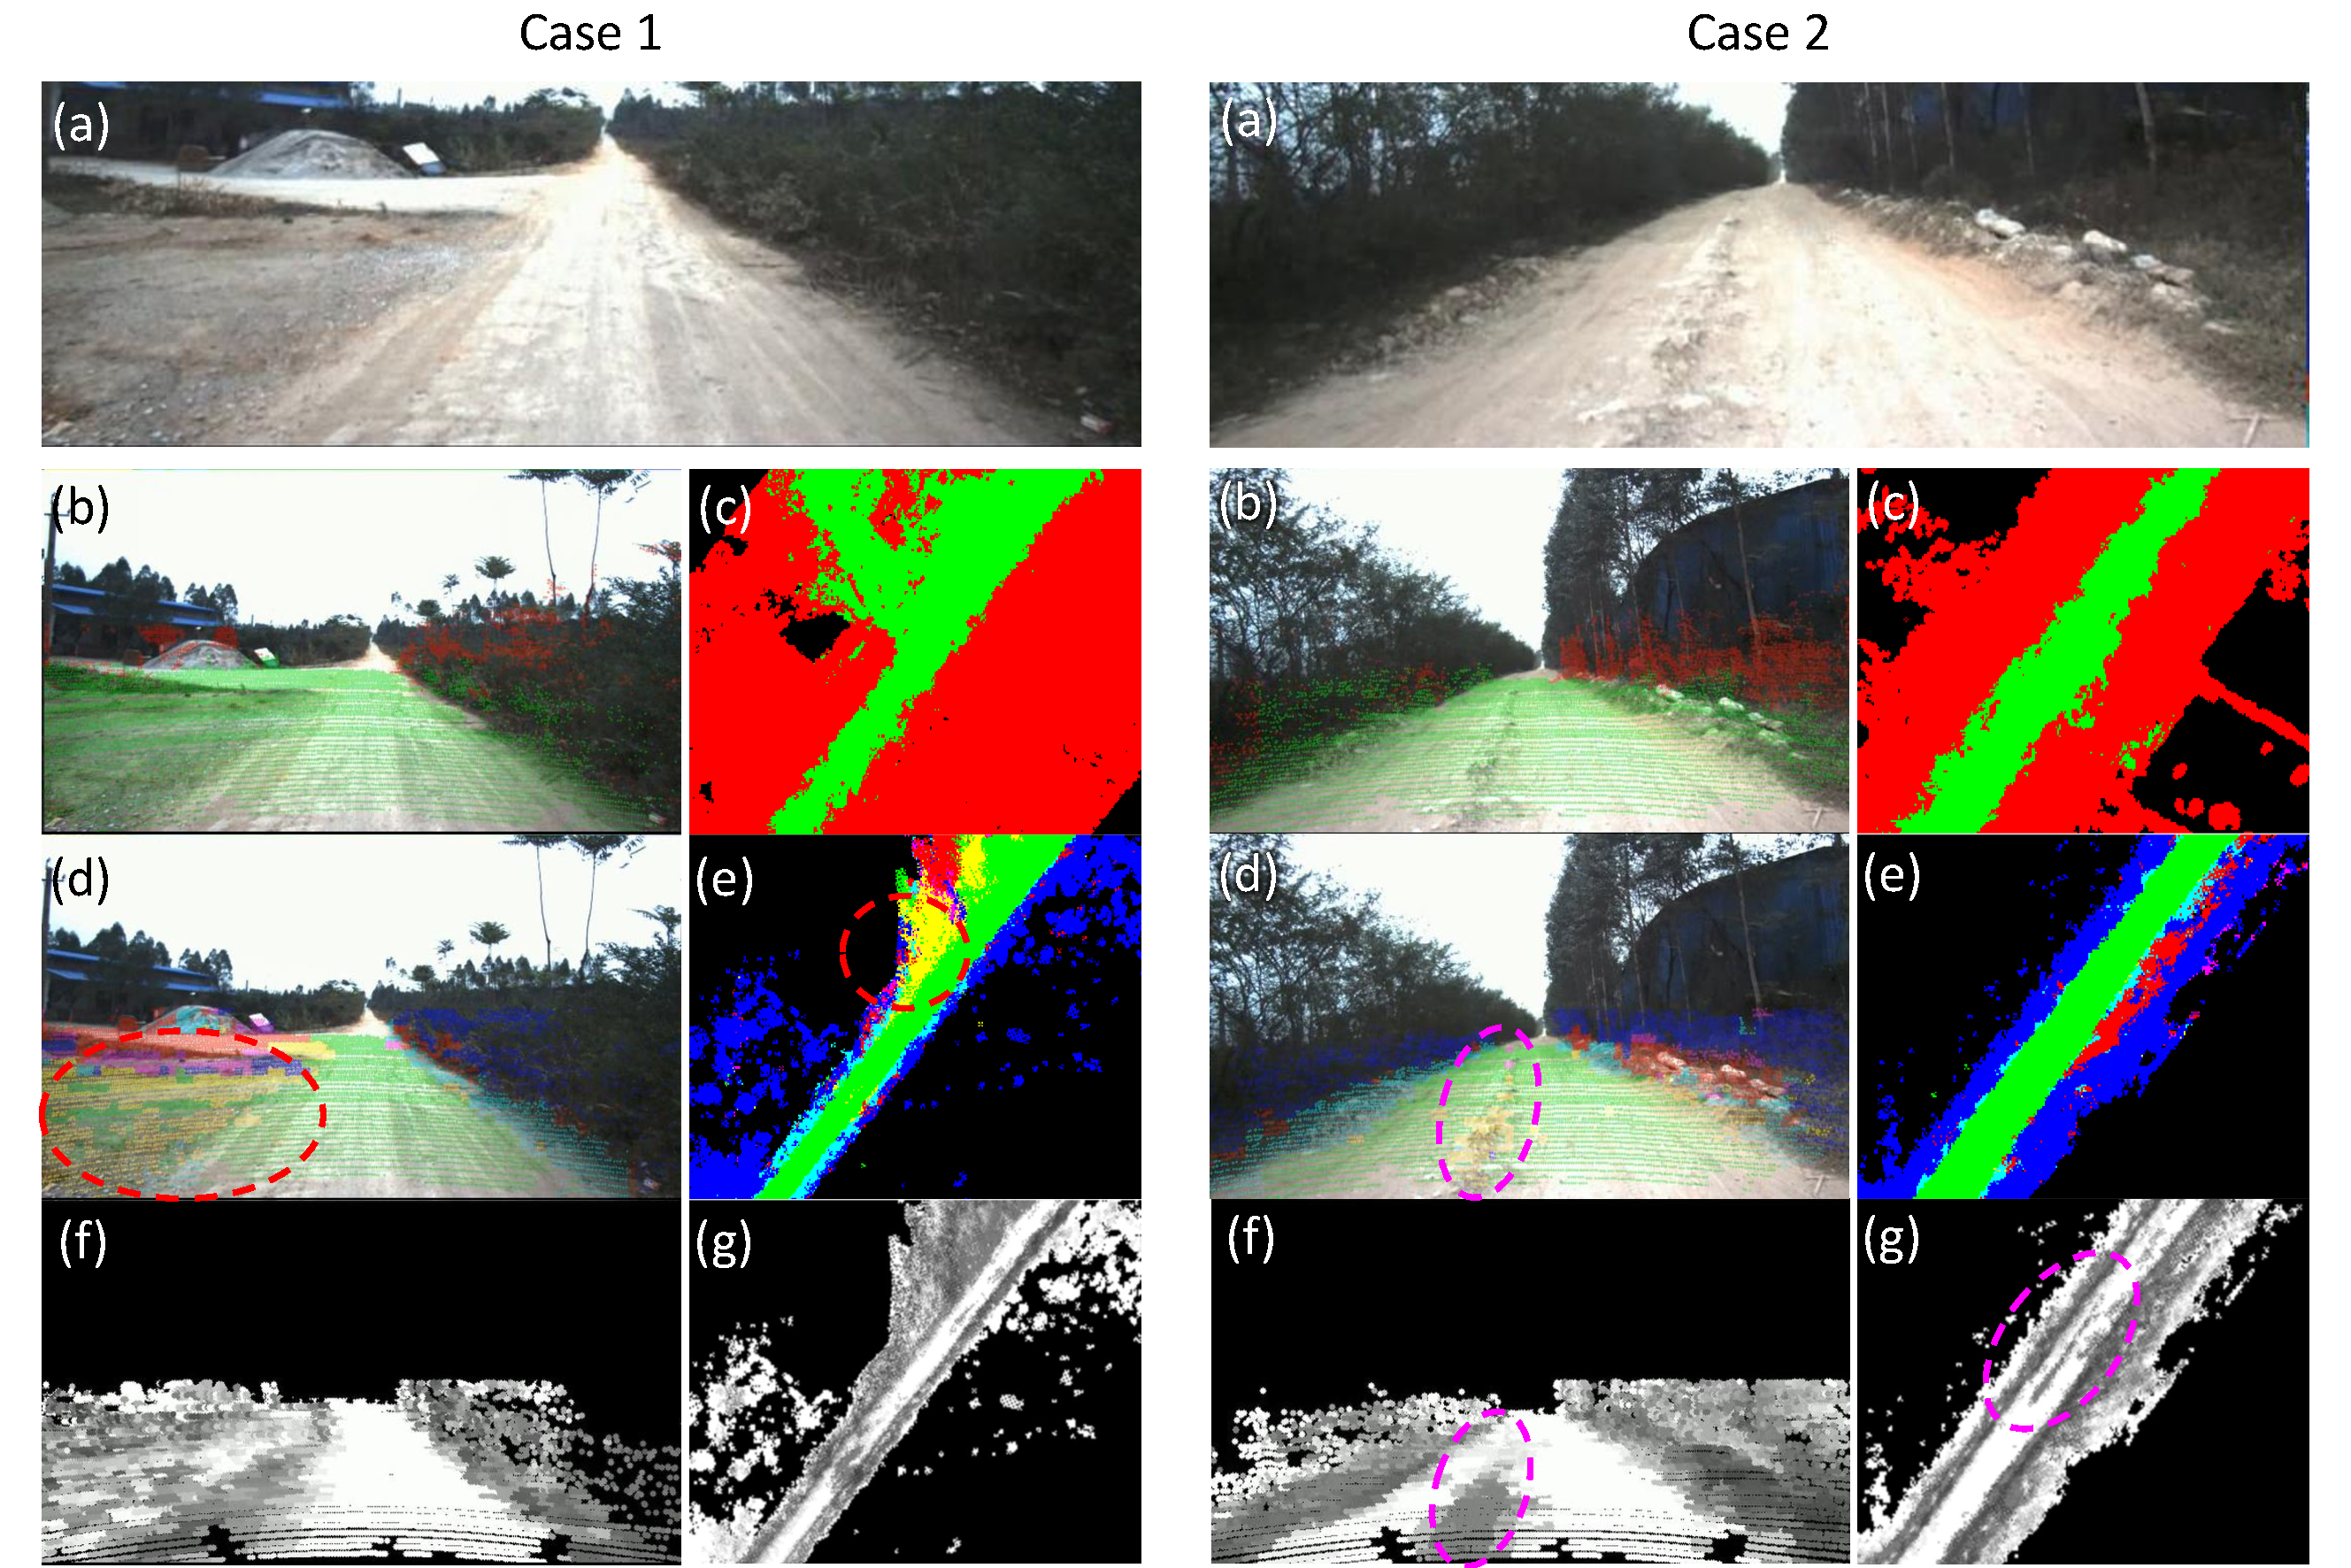
\includegraphics[width=\textwidth]{semantic_mapping.pdf}
	\caption{Case study of fine-grained semantic map and confidence map, compared with coarse-grained road extraction results. (a) video image. (b) coarse-grained segmentation. (c) coarse-grained bird's-eye-view semantic map. (d) fine-grained semantic segmentation projected by point clouds. (e) fine-grained bird's-eye-view semantic map. (f) confidence map projected on camera-view, the whiter the higher confidence. (g) bird's-eye-view confidence map.}
	\label{fig:semantic_mapping}
\end{figure*}

\subsubsection{Fine-Grained Semantic Segmentation and Mapping}
%1. 如图\ref{fig:semantic_segmentation}所示,展示了一些细粒度语义分割的结果;
%2. 为了验证细粒度语义分割的实用性,我们构建了语义地图和置信度地图(简要介绍如何建图)。结合图\ref{fig:semantic_mapping}的case分析;
%3. 借助激光雷达的数据,我们统计了各类别对应的激光点高度均值、方差的分布,结合图\ref{fig:lidar_analysis}进行说明;
%结论:我们的算法能够的到有效的细粒度语义分割结果,并可以用于语义地图、场景理解等应用中。

Due to the absent of ground truth for fine-grained off-road semantic segmentation task, we next analyze the validity of our fine-grained results through case study of semantic segmentation and mapping. Besides, we compare different categories traversability cost by additional LiDAR data. The following results are all based on the model trained by 50 frames of subset A.

\begin{figure*}[]
	%	\vspace{-2mm}
	\centering
	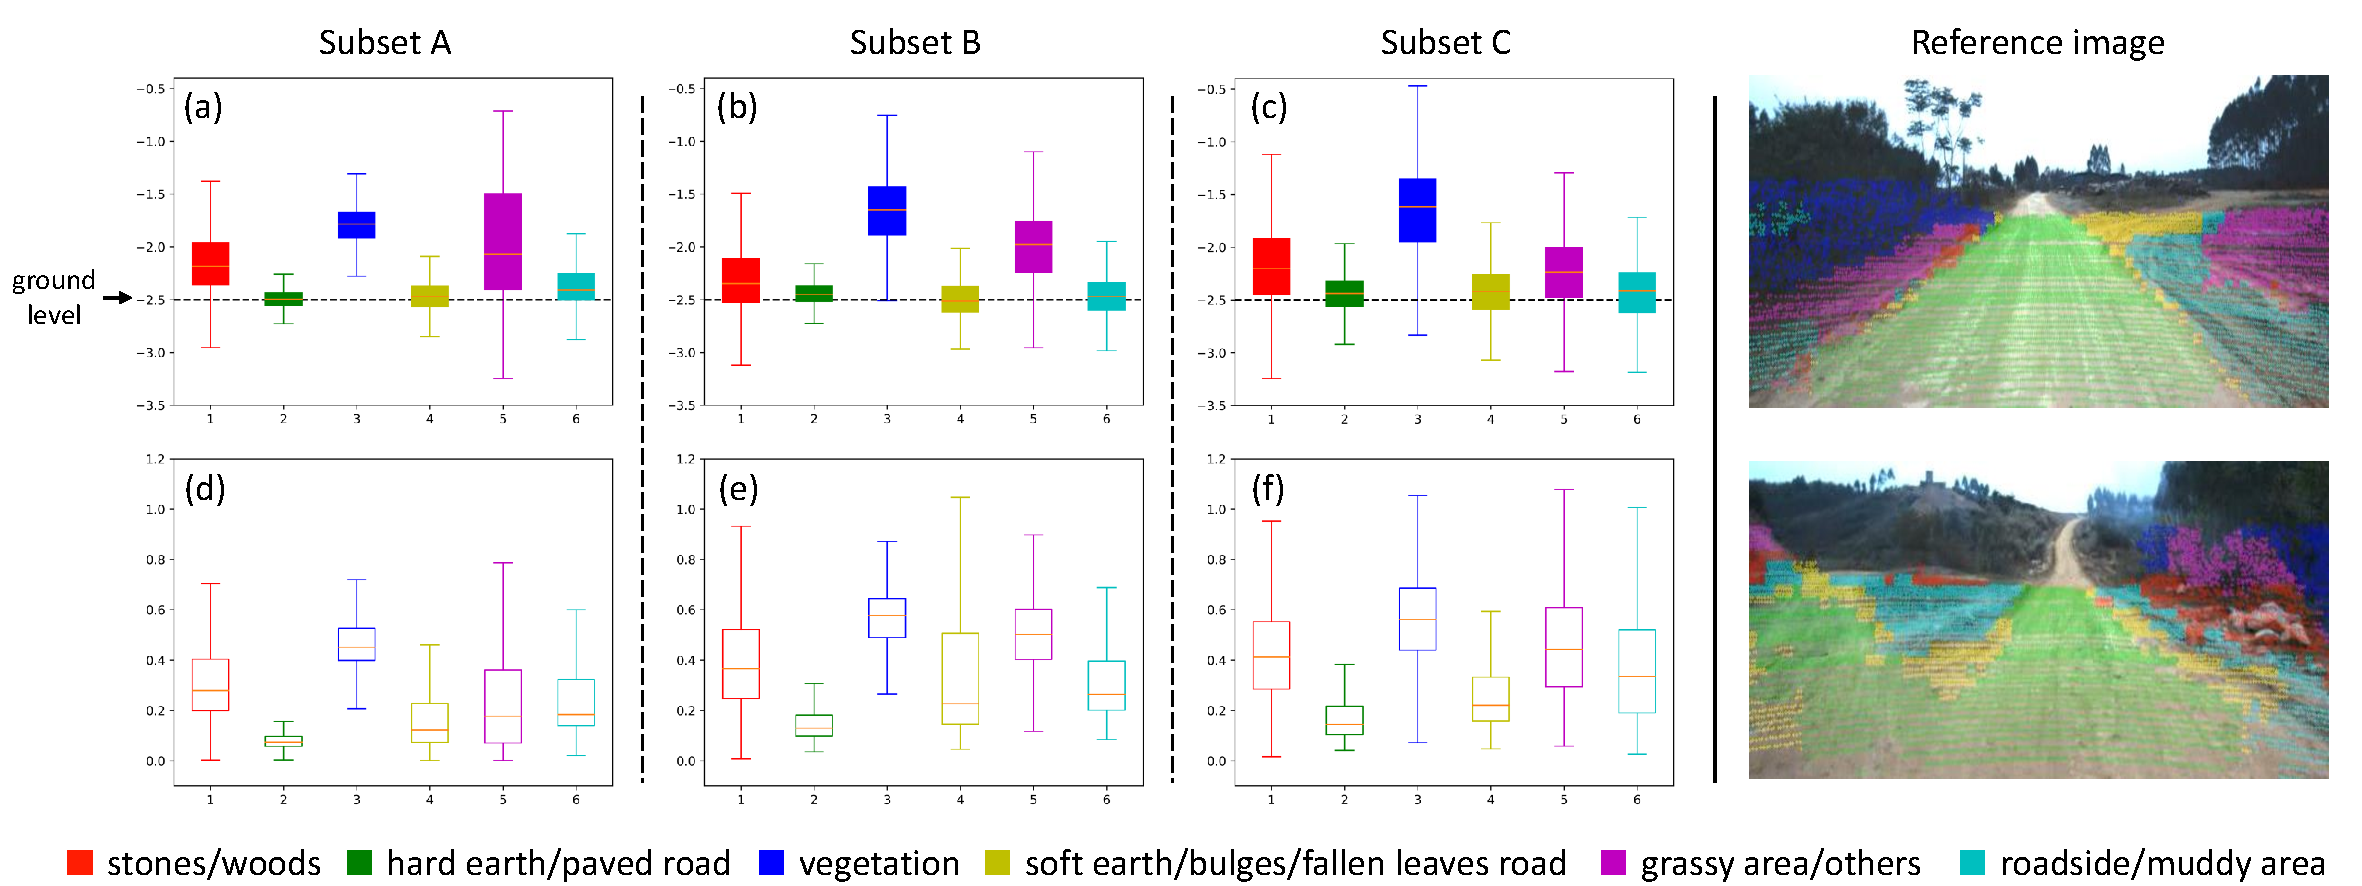
\includegraphics[width=\textwidth]{lidar_analysis.pdf}
	\caption{Traversability analysis of semantic clusters based on point clouds. (a-c) boxplots of points average height, indicate height distribution of different categories. (d-f) boxplots of points height variance, indicate surface flatness and traversability cost. }
	\label{fig:lidar_analysis}
\end{figure*}

Fig. \ref{fig:semantic_segmentation} shows some cases of fine-grained semantic segmentation. This work focuses on off-road traversability analysis, so we do not pay attention to the sky area, and only bottom half of the image are predicted for simplicity. The semantic labels are not pre-assigned, we can find some uniform semantic meanings through these concrete cases. For example, green indicates hard earth road and paved road, blue pixels are vegetation, yellow pixels are road with fallen leaves or muddy area, red pixels are stones or woods, etc. Different colors represent different clusters, and they can generally distinguish diverse semantic meanings.

To evaluate the overall performance and consistence of the fine-grained prediction on continuous video frames, we make semantic maps and confidence maps as described in Sec. \ref{3_CSS}. As shown in Fig. \ref{fig:semantic_mapping}(d)(e), our fine-grained predictions can label the roadside area (yellow) with higher traversability cost than middle road (green), while the traditional coarse-grained region grow method is unable to distinguish them. In Fig. \ref{fig:semantic_mapping}(case 2), let us pay attention to bumps in the middle of the road, which is a hard case. Although it has been separated in the single frame prediction in Fig. \ref{fig:semantic_mapping}(d), its segmentation is not stable enough to obtain majority votes in the semantic map. The good news is, confidence map in (f)(g) can be helpful to distinguish this subtle traversability difference, where the bumps area are darker than other well-travelled road.

More than case study of fine-grained semantic, segmentation, a statistical traversability analysis is provided in Fig. \ref{fig:lidar_analysis}, which is based on 3D point clouds with labels projected from fine-grained image semantic segmentation. By the way, the semantic meanings of color table is not pre-defined, but concluded from our model's predictions.
In Fig. \ref{fig:lidar_analysis}(a-c), it is obvious that green, yellow and cyan are mainly distribute around the ground level, which are three primary road types. Furthermore, in Fig. \ref{fig:lidar_analysis}(d-f), we can find their different traversability cost, where green points have the narrowest variance distribution, corresponding to the most well-travelled paved road and hard earth road. Yellow and cyan boxes are longer, indicating more bumpy road surface. They are mainly soft earth, bumps or muddy area at the roadside. Blue boxes are mostly bushes and trees, with the highest average height and traversability cost, which is in accord with boxplots distribution. In summary, the statistical analysis of additional 3D LiDAR data can prove the validity of our fine-grained off-road semantic segmentation.


\subsection{Challenges}
\begin{figure*}[]
	%	\vspace{-2mm}
	\centering
	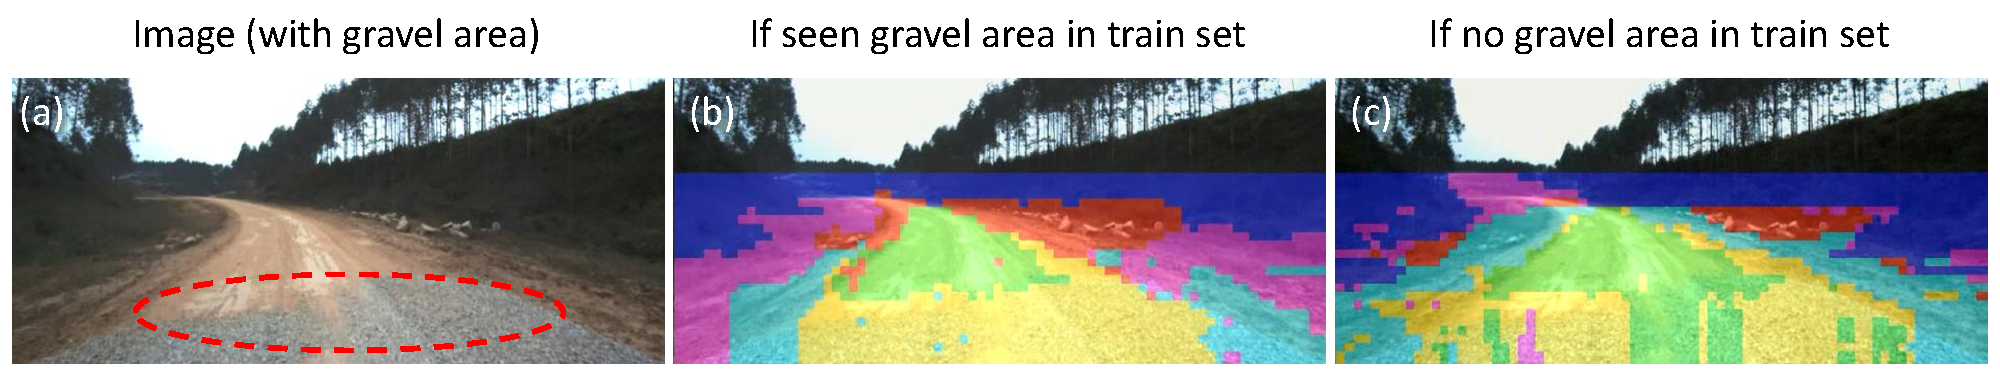
\includegraphics[width=\textwidth]{challenges.pdf}
	\caption{Challenging case: when meeting unseen semantic categories.}
	\label{fig:challenges}
\end{figure*}
%1. 预测结果连续性不够好且计算复杂度高:目前添加背景引入上下文信息的方式比较简单,预测过程中滑动窗逐个预测patch类别,并没有显式地用到一致性先验;将来需要探究如何利用时空一致性优化性能和计算效率。
%2. 没有见过的路面材质/OOD样本:目前的方法是根据K-Means结果强行并入某一类,将来需要进一步探究如何让算法主动发现OOD样本,并请求人工标注,使得模型可以增量式学习、更新。
Currently, there are still some challenges for the proposed method. Firstly, the current pipeline to obtain dense predictions has relatively high computational cost, which can be optimized by temporal and spatial consistency in future works.
The second one is unseen semantic categories, or called out of distribution (OOD) samples, as shown in Fig. \ref{fig:challenges}. The current pipeline will not discriminate unseen category samples, but simply classified them into existing clusters, which may lead to confused predictions as Fig. \ref{fig:challenges}(c). To minimize labor cost, the OOD sample detection and incremental training mechanism deserve to be explored in our future works.



\section{CONCLUSIONS}	\label{conclusions}

\addtolength{\textheight}{-12cm}   % This command serves to balance the column lengths
                                  % on the last page of the document manually. It shortens
                                  % the textheight of the last page by a suitable amount.
                                  % This command does not take effect until the next page
                                  % so it should come on the page before the last. Make
                                  % sure that you do not shorten the textheight too much.

%%%%%%%%%%%%%%%%%%%%%%%%%%%%%%%%%%%%%%%%%%%%%%%%%%%%%%%%%%%%%%%%%%%%%%%%%%%%%%%%



%%%%%%%%%%%%%%%%%%%%%%%%%%%%%%%%%%%%%%%%%%%%%%%%%%%%%%%%%%%%%%%%%%%%%%%%%%%%%%%%



%%%%%%%%%%%%%%%%%%%%%%%%%%%%%%%%%%%%%%%%%%%%%%%%%%%%%%%%%%%%%%%%%%%%%%%%%%%%%%%%
%\section*{APPENDIX}

%Appendixes should appear before the acknowledgment.

%\section*{ACKNOWLEDGMENT}

%The preferred spelling of the word ÒacknowledgmentÓ in America is without an ÒeÓ after the ÒgÓ. Avoid the stilted expression, ÒOne of us (R. B. G.) thanks . . .Ó  Instead, try ÒR. B. G. thanksÓ. Put sponsor acknowledgments in the unnumbered footnote on the first page.



%%%%%%%%%%%%%%%%%%%%%%%%%%%%%%%%%%%%%%%%%%%%%%%%%%%%%%%%%%%%%%%%%%%%%%%%%%%%%%%%

%References are important to the reader; therefore, each citation must be complete and correct. If at all possible, references should be commonly available publications.



\bibliographystyle{IEEEtran}
\bibliographystyle{unsrt}
\bibliography{root}

%\begin{thebibliography}{99}
%
%\bibitem{c1} G. O. Young, ÒSynthetic structure of industrial plastics (Book style with paper title and editor),Ó 	in Plastics, 2nd ed. vol. 3, J. Peters, Ed.  New York: McGraw-Hill, 1964, pp. 15Ð64.
%
%\end{thebibliography}




\end{document}
